% Unofficial Princeton Poster Template
% https://github.com/andiac/gemini-cam
% a fork of https://github.com/anishathalye/gemini

\documentclass[final,35pt]{beamer}

% ====================
% Packages
% ====================

\usepackage[T1]{fontenc}
\usepackage{lmodern}
% \usepackage[size=custom,width=110,height=82.5,scale=1.0]{beamerposter}
\usepackage[size=custom,width=90,height=130,scale=1.0]{beamerposter}
\usetheme{gemini}
\usecolortheme{tud}
\usepackage{graphicx}
\usepackage{booktabs}
\usepackage{tikz}
\usepackage{pgfplots}
\pgfplotsset{compat=1.14}
\usepackage{anyfontsize}
\usepackage{caption}
\usepackage{multicol}
\usepackage{multirow}
\usepackage{tcolorbox}
\usepackage{wrapfig}
\usepackage{setspace}
\usepackage[table,xcdraw]{xcolor}
% \usepackage[table]{xcolor}
% \usepackage{colortbl}

% ====================
% Lengths
% ====================

% If you have N columns, choose \sepwidth and \colwidth such that
% (N+1)*\sepwidth + N*\colwidth = \paperwidth
\newlength{\sepwidth}
\newlength{\colwidth}
\setlength{\sepwidth}{0.025\paperwidth}
\setlength{\colwidth}{0.4625\paperwidth}

\onehalfspacing

\newcommand{\separatorcolumn}{\begin{column}{\sepwidth}\end{column}}

\newcommand{\todo}[1]{\textcolor{red}{TODO: #1}}

\definecolor{green}{RGB}{0,155,119}
% \newcolumntype{C}[1]{>{\columncolor{lightgreentud}[#1]\centering\arraybackslash}m{#1}}
% ====================
% Title
% ====================

\title{Control using Spiking Neural Networks Trained with Reinforcement Learning and Surrogate Gradients}

\author{K. Van den Berghe, S. Stroobants, G.C.H.E. de Croon}

\institute[shortinst]{Delft University of Technology}


% \institute[shortinst]{\inst{1} Harvard University \samelineand \inst{2} Another Institute}
% ====================
% Footer (optional)
% ====================

\footercontent{    
   ICNCE 2024 \hfill \hfill
  \href{mailto:k.c.m.vandenberghe@student.tudelft.nl}{k.c.m.vandenberghe@student.tudelft.nl}}
% (can be left out to remove footer)

% ====================
% Logo (optional)
% ====================
% Refer to https://github.com/k4rtik/uchicago-poster
% use this to include logos on the left and/or right side of the header:
\logoright{
\includegraphics[height=2cm]{logos/MAVLab_logo.png}}
\logoleft{
\includegraphics[height=7cm]{logos/TUDelft-logo_black.png}}

% ====================
% Body
% ====================

\begin{document}



\begin{frame}
\begin{columns}[t]
\separatorcolumn

\begin{column}{\colwidth}

\begin{block}{{\fontsize{48}{24}\selectfont Motivation}}
% The rapid growth of artificial intelligence and machine learning has resulted in increasingly complex and large models in pursuit of higher accuracy and range of use cases. This has raised the desire to explore new resource-efficient and scalable computing architectures. Neuromorphic computing has emerged as a promising approach that could provide increased scalability, energy efficiency and enable real-time embodied computation by mimicking biological neural networks in novel computing architectures. \\
% Despite its promises, progress in the field of neuromorphic research is impeded due to the absence of fair and widely-adopted objective metrics and benchmarks. Without such benchmarks, the validity of neuromorphic solutions cannot be directly quantified, hindering the research community from measuring technological advancement.\\
% Standard and rigorous benchmarking is necessary for the neuromorphic community to objectively assess and compare the achievements of novel approaches, and make evidence-based decisions on which directions show promise for achieving breakthrough efficiency, speed, and intelligence, thereby helping to focus research and commercialization efforts on techniques that concretely improve on prior work and conventional computing. Neuromorphic benchmarks have been previously proposed for classical vision and audition tasks, open-loop and closed-loop tasks, and for SNN simulator performance assessment.
{
Deep reinforcement learning (RL) enables autonomous agents to achieve human-level performance in complex tasks through interaction with their environment. When deploying agents on edge devices, we are limited by computational and energy resources. Neuromorphic solutions such as spiking neural networks (SNNs) offer a promising avenue for improved energy efficiency.\\
}
\vspace{1cm}
{
We investigate \textbf{efficient deep spiking reinforcement learning}. Using \textbf{surrogate gradient} backpropagation through time, enabled by \textbf{training on sequences}, we take the networks' inherent memory into account. 
}
\end{block}
\vspace{1.5cm}
% The introduction of \textbf{surrogate gradients} has removed many obstacles to training SNNs. By relying on backpropagation, we can leverage years of research in the machine learning domain and apply reinforcement learning methods.
% \end{block}
% \vspace{1.5cm}
% Current attempts to train SNNs with \textbf{conventional RL} methods involve training on \textbf{single state-action-state transitions}, which requires rate coding or passing an observation through the network multiple times. This approach impedes the network's ability to learn temporal relations and potentially decreases energy efficiency. \textbf{This work} focuses on \textbf{training on sequences} rather than single transitions.

\begin{block}{{\fontsize{48}{40}\selectfont Methods}}

{
\begin{itemize}
    \item \textbf{Advantage Actor Critic (A2C):} an \textbf{on-policy} RL algorithm. Instead of batching the interactions of multiple actors to single transitions, the network trains on \textbf{full sequences}. 

    \vspace{1cm}
    \item \textbf{Spiking neural network:} continuous data is directly passed to the first hidden layer by using a linear encoding layer. The output of the network is defined by the membrane potentials of the final layer, which is a non-spiking LI neuron. The neurons in the hidden layers are \textbf{LIF neurons}.

    \vspace{1cm}
    \item \textbf{Target tasks:} two tasks were analyzed, the \textbf{carpole task} and a \textbf{drone landing task}. In cartpole, the net controls left and right movement. In the drone landing task, the network applies a throttle command based on sonar altitude inputs. 
\end{itemize}
}
\vspace{0.25cm}

% \begin{tcolorbox}[left=12pt, right= 12pt, top=12pt, bottom=12pt, arc=0pt, outer arc=0pt, colback = tudlightblue]
% Based on these three challenges, an open community of researchers interested in neuromorphics from academia and industry have developed \textbf{NeuroBench}. The benchmark framework is \textbf{generally applicable} to varied solution types, associated with \textbf{open-source benchmark tools}, and plans to \textbf{continually grow} in tasks and features over time. 
% \end{tcolorbox}

\end{block}

\vspace{1.5cm}

\begin{figure}[h!]
    \centering
    \begin{minipage}{0.45\textwidth}
        \centering
        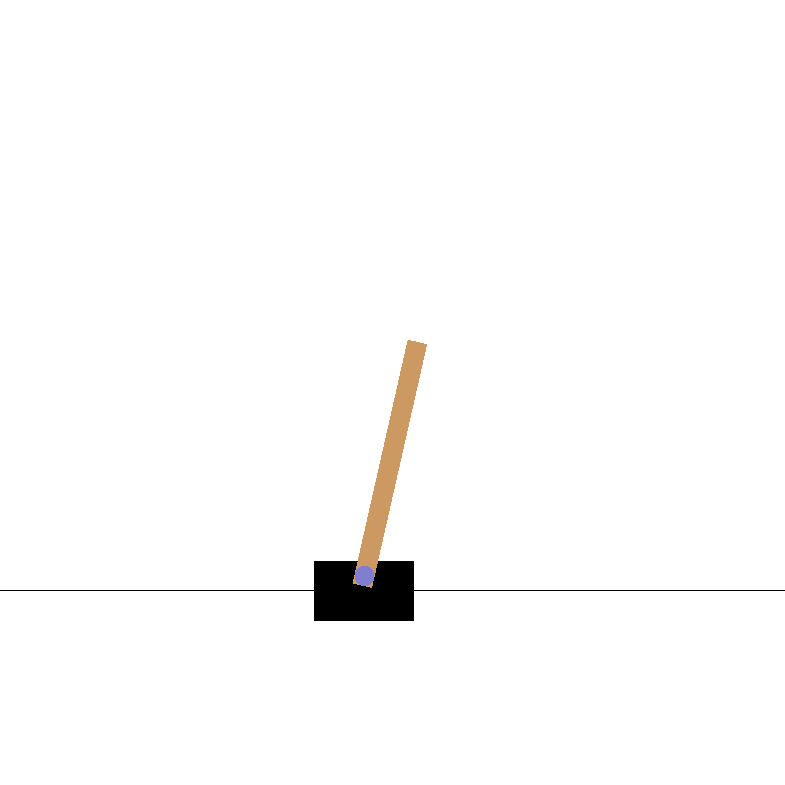
\includegraphics[width=\textwidth]{figures/cartpole.png}
        \caption{{\fontsize{28}{40}\selectfont The Cartpole environment from Gymnasium.}}
        \label{fig:image1}
    \end{minipage}\hfill
    \begin{minipage}{0.45\textwidth}
        \centering
        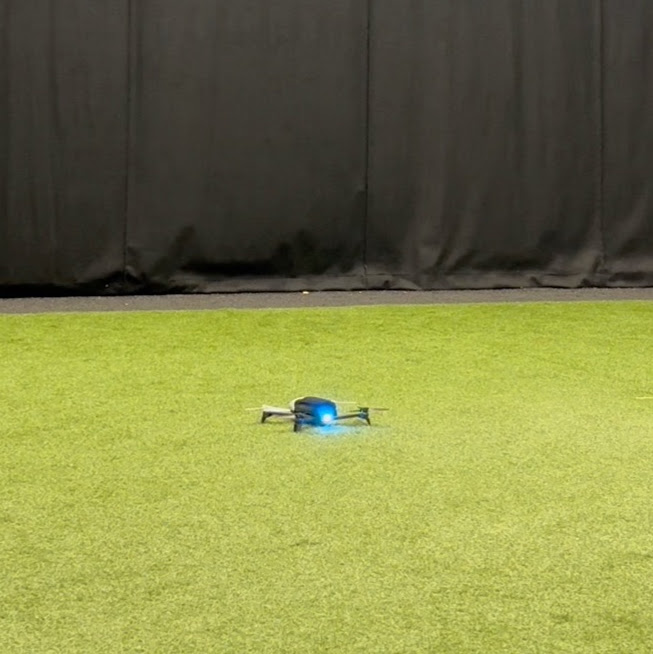
\includegraphics[width=\textwidth]{figures/bebop2.JPG}
        \caption{{\fontsize{28}{40}\selectfont The Parrot Bebop 2 drone is used for evaluation of the drone environment.}}
        \label{fig:image2}
    \end{minipage}
\end{figure}
\vspace{1.5cm}

  \begin{block}{{\fontsize{48}{40}\selectfont Training and Pruning Process}}

The SNN converges slower and noisier than comparable ANN. When the leakage can be learned, the network \textbf{learns to disregard the temporal dimension} (complete leakage). In a second experiment, the leak was fixed to a non-zero value.
\begin{figure}
    \centering
    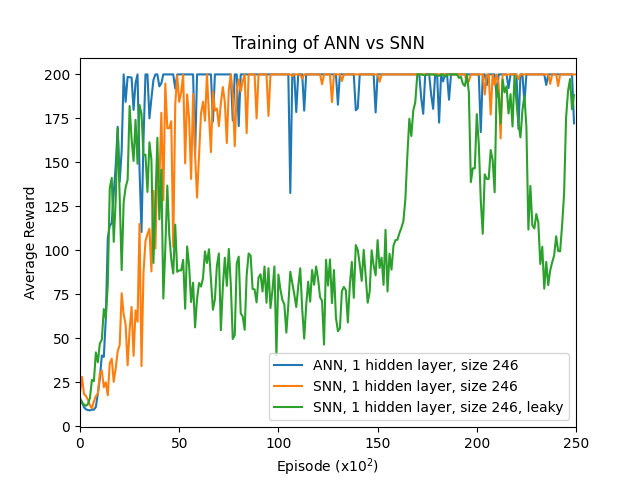
\includegraphics[width=.5\textwidth]{figures/training_3models.png}
    \caption{{\fontsize{28}{40}\selectfont  Training of an ANN and SNN with one hidden layer
of size 246. The first SNN learns to reduce β to zero. The
second SNN has a fixed leak, β = 0.65.}}
    \label{fig:training}
\end{figure}
% \begin{wrapfigure}{l}{width=.45\textwidth}    
% % \centering
%     \begin{center}
%         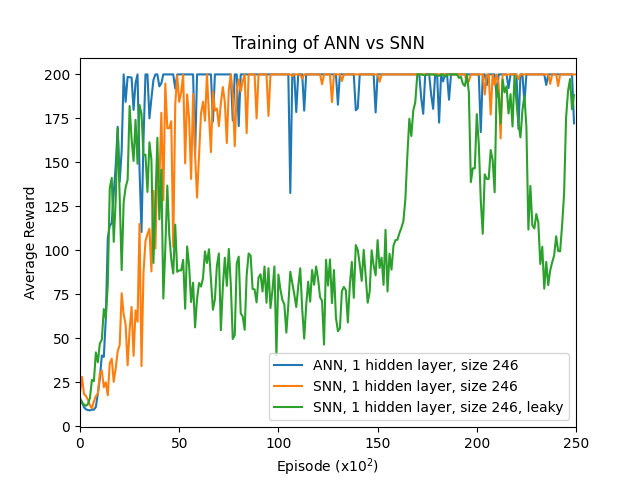
\includegraphics[width=.48\textwidth]{figures/training_3models.png}
%     \end{center}
%     \caption{{\fontsize{28}{40}\selectfont  Training of an ANN and SNN with one hidden layer
% of size 246. The first SNN learns to reduce β to zero. The
% second SNN has a fixed leak, β = 0.65.}}
%     \label{fig:training}
% \end{wrapfigure}

{
SNNs were \textbf{pruned based on activity}, removing dead and saturated neurons. This leads to reduced models.
\begin{itemize}
    \item Hidden layer of \textbf{only 11 neurons} for the model with full leakage.
    \item Hidden layer of \textbf{only 21 neurons} for the model which has a fixed leakage.
\end{itemize}
These reduced models showed little decrease in performance.
   }
  \end{block}
\end{column}
% \end{column}
\separatorcolumn

\begin{column}{\colwidth}



  \begin{block}{{\fontsize{48}{40}\selectfont NeuroBench Results}}
  {
NeuroBench \cite{yik2024neurobench} is a community driven neuromorphic benchmarking framework. The complexity metrics provided by the benchmark include the synaptic operations, activation sparsity and footprint. The performance of the algorithms are described by the reward and the risk, representing the $5\%$ worst performing interactions.
}

\begin{table}[h]
\centering
\renewcommand{\arraystretch}{1.5}
\begin{tabular}{c|c|c|c|c|c} \thickhline
 Baseline & ANN & SNN & SNN_{leaky} & SNN_{p} & SNN_{leaky, p}\\ \hline
 Reward ($\mu$ $\pm$ $\sigma$) & 1744 $\pm$ 1385 & 1620 $\pm$ 1600 & 232 $\pm$ 65 & \textbf{\color{green}1570 $\pm$ 1480} & 200 $\pm$ 64 \\
 Risk & 190 & 148 & 152 & \textbf{\color{green}140} & 73 \\ \hline
 Footprint (bytes) & $7.9 \times 10^3$ & $7.9 \times 10^3$ & $7.9 \times 10^3$ & \textbf{\color{green}360} & 640 \\
 Activation Sparsity & 0.0 & 0.68 & 0.92 & \textbf{\color{green}0.49} & 0.65 \\
 SynOps Dense & $1.7 \times 10^{3}$ & $1.7 \times 10^{3}$ & $1.7 \times 10^{3}$ & \textbf{\color{green}66} & 126 \\
 SynOps Eff\_MACs & $1.5 \times 10^{3}$ & $0.9 \times 10^{3}$ & $0.9 \times 10^{3}$ & \textbf{\color{green}44} & 84 \\
 SynOps Eff\_ACs & 0 & 238 & 59 & \textbf{\color{green}12} & 16 \\ \thickhline
\end{tabular}
\caption{{\fontsize{28}{40}\selectfont NeuroBench results for the single layer ANN and SNNs (regular, leaky, pruned (p), and leaky pruned (p) controlling the CartPole task.}}
\label{tab:combined_results}
\end{table}
{
The pruned spiking neural networks allow for an impressive \textbf{reduction in synaptic operations for a relatively small decrease in performance}. Pruning efforts for the ANN were unable to achieve similar characteristics.
   
}

  \end{block}



  \begin{block}{{\fontsize{48}{40}\selectfont Noise Robustness}}
  {
The 5 different models, with artificial neurons, spiking neurons with and without temporal capabilities, are compared upon injection of Gaussian noise into the input data. 
}
\begin{figure}
    \centering
    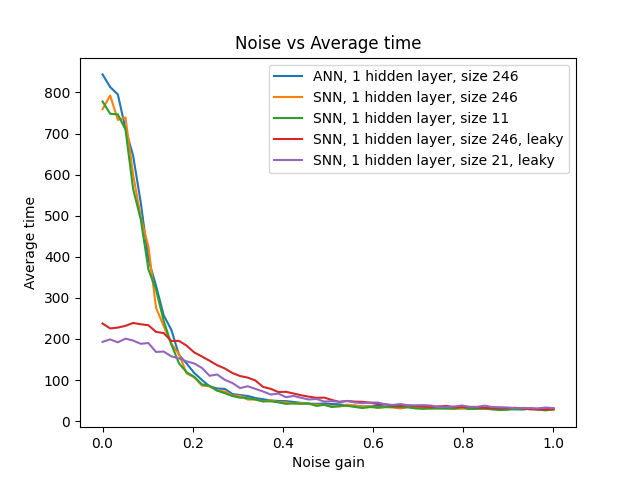
\includegraphics[width=.85\textwidth]{figures/Noise_Robustness_5Models.png}
    \caption{{\fontsize{28}{40}\selectfont Noise robustness analysis of the artificial, and spiking models.}}
    \label{fig:enter-label}
\end{figure}
{
\begin{itemize}
    \item \textbf{Pruned models achieved similar performance} to their original models independent of noise injection.
    \item \textbf{Leakage enables the models to perform more robustly} to noisy sensory data.
\end{itemize}

}
  \end{block}

\vspace{-0.75cm}

\begin{block}{{\fontsize{48}{40}\selectfont Deployment on a UAV}}
{
A model with two hidden layers of 32 LIF neurons, uses noisy sonar altitude measurements, requiring the network to estimate velocity. The net controls the throttle setting, to successfully land a UAV.
}
\begin{figure}
    \centering
    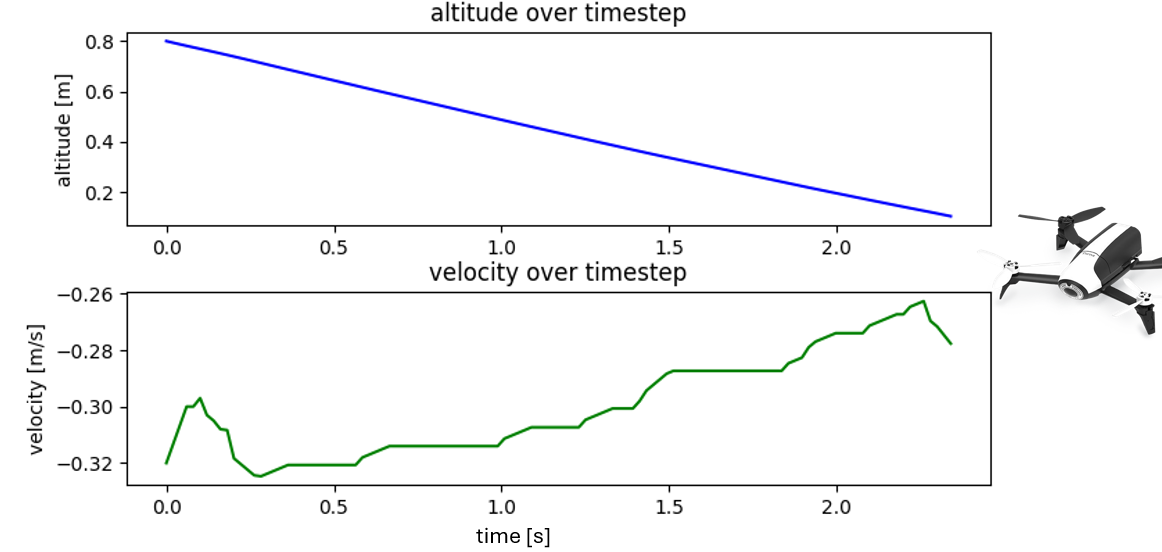
\includegraphics[width=.8\textwidth]{figures/drone_landing.png}
    \caption{{\fontsize{28}{40}\selectfont An SNN trained with the previously described pipeline can successfully land the Parrot Bebop 2 drone, decreasing velocity as it nears the ground.}}
    \label{fig:enter-label}
\end{figure}
\end{block}

\vspace{-0.5cm}

%   \begin{block}{{\fontsize{48}{40}\selectfont Future Work}}
%   {
% While it is possible to train an SNN by modifying the A2C algorithm to train on sequences and using the surrogate gradient for backpropagation, the SNN fails to fully exploit temporal dynamics. In future work, I would like to explore how to\textbf{ train an SNN to exploit temporal dynamics with RL} and attempt to \textbf{combine the fast learning of ANN as a critic or guiding policy with a SNN-based actor} in RL.
% }

%   \end{block}
%   \begin{block}{{\fontsize{48}{40}\selectfont References}}
%       \vspace{.3cm}\footnotesize{\bibliographystyle{plain}\bibliography{poster}}
%   \end{block}

\end{column}

\separatorcolumn
\end{columns}
  \begin{block}{{\fontsize{48}{40}\selectfont Future Work}}
  {
While it is possible to train an SNN by modifying the A2C algorithm to train on sequences and using the surrogate gradient for backpropagation, the SNN fails to fully exploit temporal dynamics. In future work, I would like to explore how to\textbf{ train an SNN to exploit temporal dynamics with RL} and attempt to \textbf{combine the fast learning of ANN as a critic or guiding policy with a SNN-based actor} in RL.
}

  \end{block}
  \begin{block}{{\fontsize{48}{40}\selectfont References}}
      \vspace{.3cm}\footnotesize{\bibliographystyle{plain}\bibliography{poster}}
  \end{block}
\end{frame}

\end{document}
